In den entsprechenden Papern zu diesem Thema wurden meist Beispiele aus dem medizinischen Bereich mit �rzten, Patienten, Untersuchungen und mehr gew�hlt. Wir haben uns f�r ein anderes Feld entschieden: den Flugverkehr. Hier existieren viele verschiedene Daten, die je nach Angreifermodell und Nutzer zu sch�tzen sind. Eine Fluggesellschaft ist zum Beispiel daran interessiert, welche Reisende ihr Kontingent an Gep�ckst�cken beziehungsweise Gewicht �berschreiten, um ihnen beim n�chsten Flug ein teureres Ticket verkaufen zu k�nnen. Andererseits soll aber nicht f�r jeden erkennbar sein wer, wann, wohin geflogen ist.

Die von uns erdachte Datenbank besteht aus 6 Tabellen: \textit{Buchungen}, \textit{Gepaeck}, \textit{Fluege}, \textit{Reisende}, \textit{Flugzeuge} und \textit{Piloten}. Die jeweils enthaltenen Attribute sind in den Tabellen \ref{tab:SchemaBuchungen} bis \ref{tab:SchemaPiloten} zu sehen. Grau hinterlegte Attribute, h�ufig Fremdschl�ssel, m�ssen unserer Meinung nach besonders gesch�tzt werden und werden deshalb auf dem ``SmartUSB''-Stick gespeichert.

\begin{table}[H]
\centering
\begin{tabular}{|l|}
\hline
\bfseries Buchungen\\
\hline
BuchungsID\\
Datum\\
Preis\\
Flug\\
\cellcolor[rgb]{0.85,0.85,0.85}Reisender\\
\hline
\end{tabular}
\caption{Schema Buchungen}
\label{tab:SchemaBuchungen}
\end{table}

\begin{table}[H]
\centering
\begin{tabular}{|l|}
\hline
\bfseries Gepaeck\\
\hline
GepaeckID\\
Flug\\
Gewicht\\
Abgabe\\
\cellcolor[rgb]{0.85,0.85,0.85}Reisender\\
\hline
\end{tabular}
\caption{Schema Gepaeck}
\label{tab:SchemaGepaeck}
\end{table}

\begin{table}[H]
\centering
\begin{tabular}{|l|}
\hline
\bfseries Fluege\\
\hline
FlugID\\
Start\\
Ziel\\
Entfernung\\
Abflug\\
Flugzeug\\
\cellcolor[rgb]{0.85,0.85,0.85}Pilot\\
\hline
\end{tabular}
\caption{Schema Fluege}
\label{tab:SchemaFluege}
\end{table}

\begin{table}[H]
\centering
\begin{tabular}{|l|}
\hline
\bfseries Reisende\\
\hline
ReisenderID\\
Vorname\\
Name\\
Geschlecht\\
\cellcolor[rgb]{0.85,0.85,0.85}Geburtsdatum\\
\cellcolor[rgb]{0.85,0.85,0.85}Staatsbuergerschaft\\
\hline
\end{tabular}
\caption{Schema Reisende}
\label{tab:SchemaReisende}
\end{table}

\begin{table}[H]
\centering
\begin{tabular}{|l|}
\hline
\bfseries Flugzeuge\\
\hline
FlugzeugID\\
Typ\\
Reichweite\\
Sitzplaetze\\
\hline
\end{tabular}
\caption{Schema Flugzeuge}
\label{tab:SchemaFlugzeuge}
\end{table}

\begin{table}[H]
\centering
\begin{tabular}{|l|}
\hline
\bfseries Piloten\\
\hline
PilotID\\
Vorname\\
Name\\
Geschlecht\\
\cellcolor[rgb]{0.85,0.85,0.85}Geburtsdatum\\
\cellcolor[rgb]{0.85,0.85,0.85}Gehalt\\
\hline
\end{tabular}
\caption{Schema Piloten}
\label{tab:SchemaPiloten}
\end{table}

Visualisiert man die Fremdschl�sselbeziehungen zwischen den Tabellen mit Pfeilen ergibt sich die Struktur in Abbildung \ref{fig:Datenmodell}. Die hier verwendete Datenbank unterscheidet sich strukturell stark von dem Beispiel, dass die ``GhostDB''-Autoren verwendeten. Am Auff�lligsten ist das Vorhandensein von zwei ``Wurzeln''. In den zugrunde liegenden Arbeiten werden explizit nur Datenbanken in Baumstrukur, das hei�t mit einer Wurzel, vorgesehen. Dies sahen wir als Herausforderung das ``GhostDB''-System hieran zu erproben. Erstaunlicherweise entstanden dadurch kaum Probleme. In der Anfragebearbeitung waren aber teilweise zus�tzliche Schritte n�tig.

\begin{figure}[htbp]
\centering
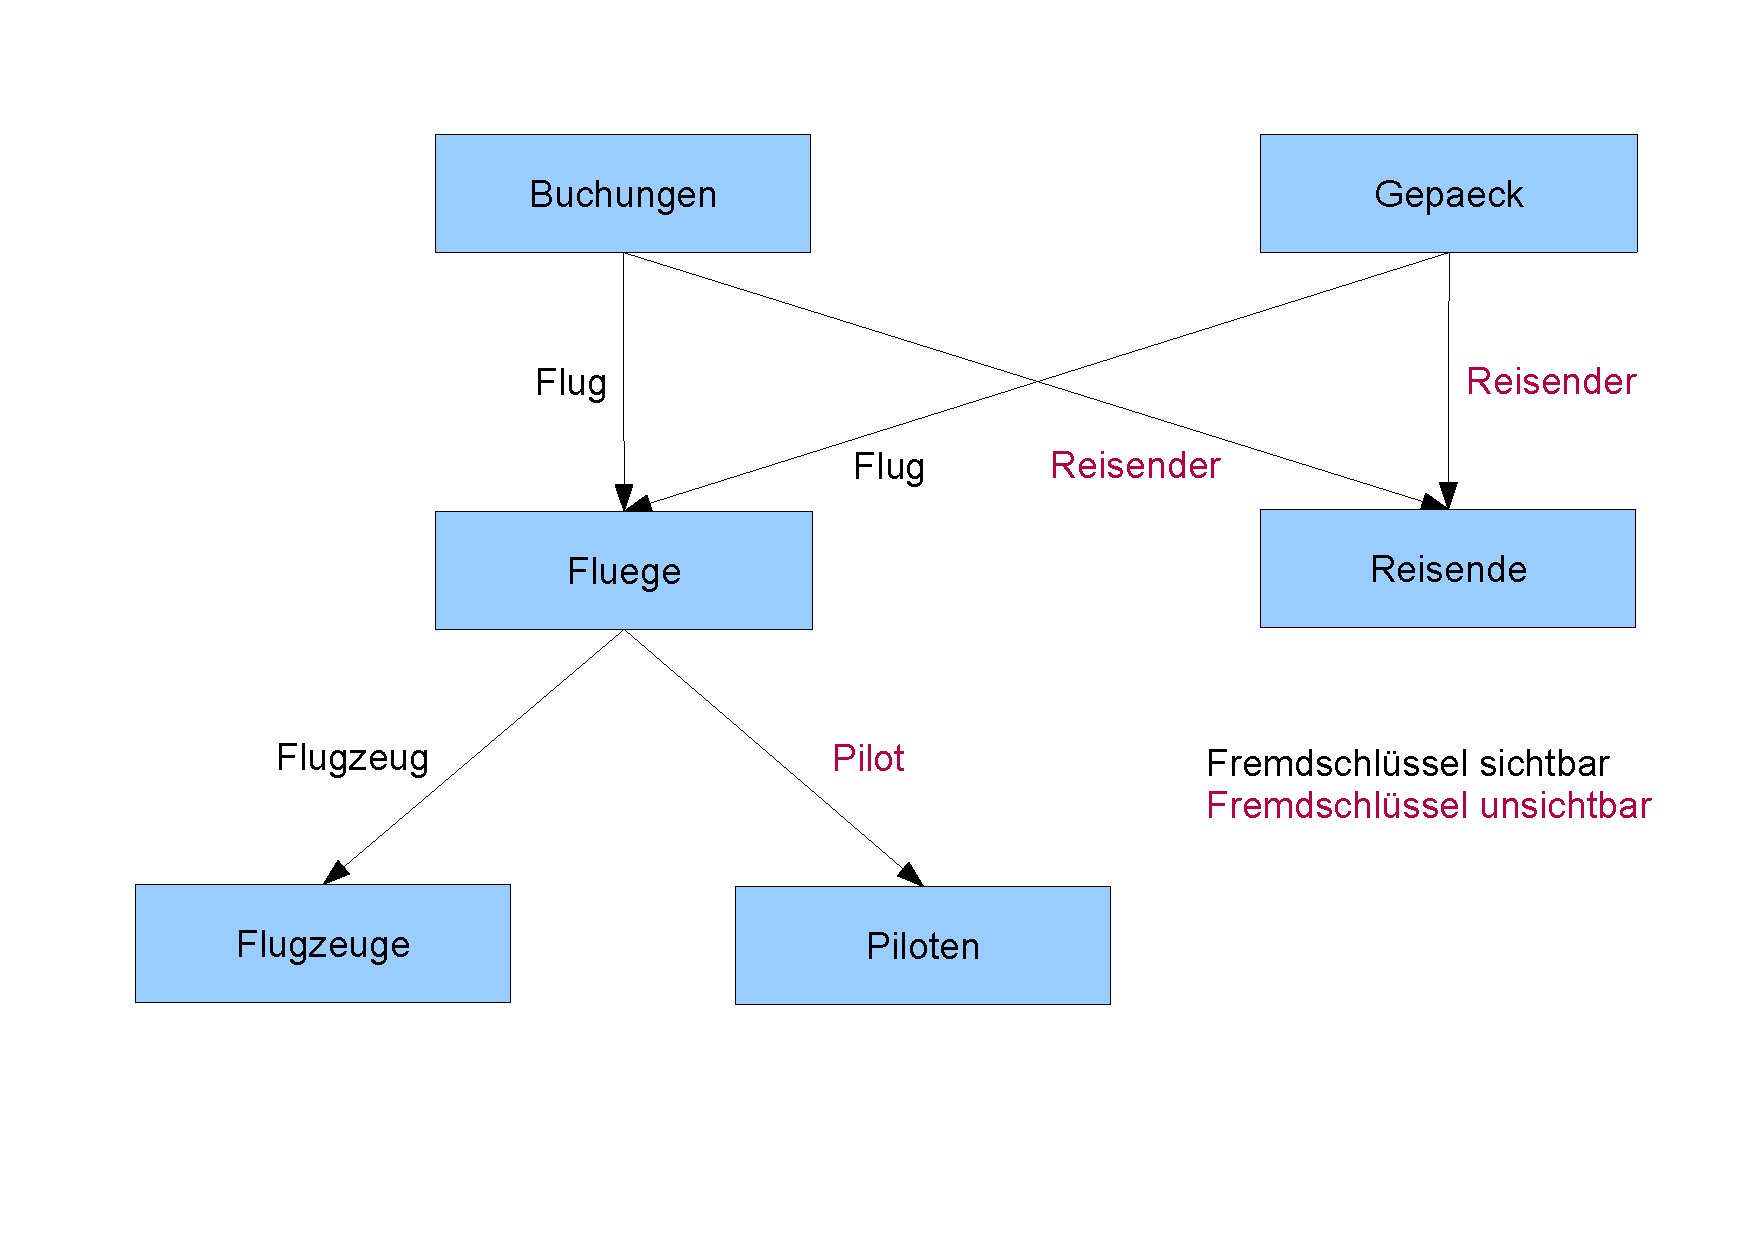
\includegraphics[width=1.00\textwidth]{img/Datenmodell.pdf}
\caption{Datenmodell}
\label{fig:Datenmodell}
\end{figure}

Um die verwendeten Strukturen, ``Subtree Key Table'' und ``Climbing Index'', ad�quat vorzustellen, haben wir die ausgedachten Tabellen mit Daten ausgef�llt. Dies ist in den Tabllen \ref{tab:Buchungen} bis \ref{tab:Piloten} dargestellt. Einige Tabellen enthalten Attribute, die nicht frei erfunden sind, insbesondere Personen und Orte. Die dabei verwendeten Quellen sind im Anhang aufgelistet.

\begin{table}[htbp]
\centering
\begin{tabular}{|c|c|c|c|c|}
\hline
\bfseries BuchungsID&\bfseries Datum&\bfseries Preis&\bfseries Flug&\bfseries Reisender\\
\hline
B01&2010-12-08&342&F13&R02\\
\hline
B02&2011-01-04&226&F09&R06\\
\hline
B03&2011-01-23&241&F06&R01\\
\hline
B04&2011-03-15&469&F09&R15\\
\hline
B05&2011-04-04&339&F02&R13\\
\hline
B06&2011-05-13&490&F13&R03\\
\hline
B07&2011-05-18&109&F10&R11\\
\hline
B08&2011-05-18&137&F15&R07\\
\hline
B09&2011-05-20&66&F13&R09\\
\hline
B10&2011-06-04&220&F08&R04\\
\hline
B11&2011-06-15&222&F15&R03\\
\hline
B12&2011-06-22&147&F06&R02\\
\hline
B13&2011-06-22&147&F06&R14\\
\hline
B14&2011-06-22&65&F06&R09\\
\hline
B15&2011-07-01&319&F01&R10\\
\hline
B16&2011-07-09&380&F14&R08\\
\hline
B17&2011-07-14&394&F03&R12\\
\hline
B18&2011-07-26&161&F15&R13\\
\hline
B19&2011-08-05&325&F15&R05\\
\hline
B20&2011-08-09&257&F05&R04\\
\hline
B21&2011-08-09&257&F05&R11\\
\hline
B22&2011-08-10&432&F09&R01\\
\hline
B23&2011-08-13&157&F14&R10\\
\hline
B24&2011-08-22&90&F08&R03\\
\hline
B25&2011-08-23&416&F09&R08\\
\hline
\end{tabular}
\caption{Buchungen}
\label{tab:Buchungen}
\end{table}

\begin{table}[htbp]
\centering
\begin{tabular}{|c|c|c|c|c|}
\hline
\bfseries GepaeckID&\bfseries Flug&\bfseries Gewicht&\bfseries Abgabe&\bfseries Reisender\\
\hline
G01&F08&14&2011-08-20 17:05&R04\\
\hline
G02&F08&10&2011-08-20 17:05&R04\\
\hline
G03&F09&15&2011-08-23 09:30&R01\\
\hline
G04&F10&16&2011-08-16 07:31&R11\\
\hline
G05&F06&14&2011-08-09 12:58&R02\\
\hline
G06&F06&21&2011-08-09 12:58&R14\\
\hline
G07&F05&14&2011-08-09 13:00&R11\\
\hline
G08&F08&20&2011-08-22 21:47&R04\\
\hline
G09&F09&20&2011-08-23 08:45&R15\\
\hline
G10&F13&15&2011-08-23 20:20&R02\\
\hline
G11&F10&11&2011-08-23 14:35&R11\\
\hline
G12&F08&21&2011-08-21 07:59&R03\\
\hline
G13&F10&23&2011-08-23 12:07&R11\\
\hline
G14&F09&14&2011-08-22 21:47&R08\\
\hline
G15&F01&12&2011-08-02 00:45&R10\\
\hline
G16&F01&21&2011-08-02 00:45&R10\\
\hline
G17&F13&17&2011-08-26 16:42&R09\\
\hline
G18&F15&21&2011-08-30 12:40&R07\\
\hline
G19&F05&22&2011-08-08 23:57&R04\\
\hline
G20&F05&25&2011-08-08 23:57&R04\\
\hline
G21&F08&10&2011-08-21 08:00&R03\\
\hline
G22&F13&22&2011-08-25 22:42&R02\\
\hline
G23&F06&25&2011-08-14 04:19&R01\\
\hline
G24&F14&18&2011-08-27 21:13&R08\\
\hline
G25&F15&16&2011-08-29 17:55&R13\\
\hline
\end{tabular}
\caption{Gepaeck}
\label{tab:Gepaeck}
\end{table}

\begin{sidewaystable}[htbp]
\centering
\begin{tabular}{|c|c|c|c|c|c|c|}
\hline
\bfseries FlugID&\bfseries Start&\bfseries Ziel&\bfseries Entfernung&\bfseries Abflug&\bfseries Flugzeug&\bfseries Pilot\\
\hline
F01&Berlin (SXF)&Antwerpen (ANR)&638&2011-08-02 04:25&A05&P03\\
\hline
F02&Berlin (SXF)&Barcelona (BCN)&1506&2011-08-05 16:10&A01&P02\\
\hline
F03&Berlin (SXF)&Chicago (ORD)&7118&2011-08-08 19:45&A02&P04\\
\hline
F04&Berlin (SXF)&Dortmund (DTM)&417&2011-08-09 04:05&A05&P02\\
\hline
F05&Berlin (SXF)&Erfurt (ERF)&236&2011-08-09 15:25&A04&P10\\
\hline
F06&Berlin (SXF)&Florenz (FLR)&968&2011-08-14 07:15&A01&P03\\
\hline
F07&Berlin (SXF)&Genf (GVA)&869&2011-08-19 15:45&A04&P08\\
\hline
F08&Berlin (SXF)&Hamburg (HAM)&275&2011-08-23 06:30&A05&P07\\
\hline
F09&Berlin (SXF)&Istanbul (IST)&1717&2011-08-23 12:25&A03&P02\\
\hline
F10&Berlin (SXF)&Jakarta (CGK)&10745&2011-08-23 15:20&A02&P06\\
\hline
F11&Berlin (SXF)&Kiew (KBP)&1227&2011-08-23 18:30&A04&P04\\
\hline
F12&Berlin (SXF)&London (LHR)&965&2011-08-26 13:20&A01&P01\\
\hline
F13&Berlin (SXF)&Madrid (MAD)&1853&2011-08-26 18:15&A03&P07\\
\hline
F14&Berlin (SXF)&New York (JFK)&6401&2011-08-29 00:30&A02&P08\\
\hline
F15&Berlin (SXF)&Oslo (OSL)&882&2011-08-30 15:20&A01&P10\\
\hline
\end{tabular}
\caption{Fluege}
\label{tab:Fluege}
\end{sidewaystable}

\begin{sidewaystable}[htbp]
\centering
\begin{tabular}{|c|c|c|c|c|c|}
\hline
\bfseries ReisenderID&\bfseries Vorname&\bfseries Name&\bfseries Geschlecht&\bfseries Geburtsdatum&\bfseries Staatsbuergerschaft\\
\hline
R01&Jacqueline&Auriol&F&1955-11-05&Franz�sisch\\
\hline
R02&Mike&Bannister&M&1969-10-24&Britisch\\
\hline
R03&Francis&Chichester&M&1939-09-17&Britisch\\
\hline
R04&Doru&Davidovici&M&1987-04-20&Rom�nisch\\
\hline
R05&Eugene Burton&Ely&M&1971-10-21&US-Amerikanisch\\
\hline
R06&Charles&Fern&M&1942-02-01&US-Amerikanisch\\
\hline
R07&Sabiha&G�k�en&F&1978-03-22&T�rkisch\\
\hline
R08&Ernst&Heinkel&M&1936-01-24&Deutsch\\
\hline
R09&Tony&Jannus&M&2008-07-22&US-Amerikanisch\\
\hline
R10&Algene&Key&M&1945-06-04&US-Amerikanisch\\
\hline
R11&Ruth Bancroft&Law&F&1984-11-19&US-Amerikanisch\\
\hline
R12&Marie&Marvingt&F&1966-02-20&Franz�sisch\\
\hline
R13&Charles&Nungesser&M&1964-03-15&Franz�sisch\\
\hline
R14&Ivy May&Pearce&F&1969-06-08&Australisch\\
\hline
R15&Harriet&Quimby&F&1980-05-01&US-Amerikanisch\\
\hline
\end{tabular}
\caption{Reisende}
\label{tab:Reisende}
\end{sidewaystable}

\begin{table}[htbp]
\centering
\begin{tabular}{|c|c|c|c|}
\hline
\bfseries FlugzeugID&\bfseries Typ&\bfseries Reichweite&\bfseries Sitzplaetze\\
\hline
A01&Airbus A300B4&6670&266\\
\hline
A02&Airbus A340-200&15000&240\\
\hline
A03&Boeing 747-200B&12700&366\\
\hline
A04&Bombardier CRJ100 LR&3710&50\\
\hline
A05&Bombardier CRJ1000&2491&100\\
\hline
\end{tabular}
\caption{Flugzeuge}
\label{tab:Flugzeuge}
\end{table}

\begin{table}[htbp]
\centering
\begin{tabular}{|c|c|c|c|c|c|}
\hline
\bfseries PilotID&\bfseries Vorname&\bfseries Name&\bfseries Geschlecht&\bfseries Geburtsdatum&\bfseries Gehalt\\
\hline
P01&John&Alcock&M&1949-11-05&3800\\
\hline
P02&Richard&Bach&M&1978-06-23&2300\\
\hline
P03&George&Cayley&M&1960-12-27&12000\\
\hline
P04&Jimmy&Doolittle&M&1964-12-14&5100\\
\hline
P05&Amelia&Earhart&F&1956-07-24&8400\\
\hline
P06&Henri&Farman&M&1974-05-26&6700\\
\hline
P07&Roland&Garros&M&1959-10-06&10000\\
\hline
P08&Hilda&Hewlett&F&1967-02-17&6700\\
\hline
P09&Amy&Johnson&F&1948-07-01&8300\\
\hline
P10&Fred&Key&M&1945-06-04&6000\\
\hline
\end{tabular}
\caption{Piloten}
\label{tab:Piloten}
\end{table}
